\documentclass[12pt]{article}
\usepackage[utf8]{inputenc}
\usepackage[T5]{fontenc}
\usepackage{graphicx,a4wide,framed,amssymb}
\usepackage{tikz}
\usetikzlibrary{decorations,decorations.pathmorphing,shadows}

\newcommand{\source}[1]{\begin{flushright}\emph{[#1]}\end{flushright}}

\newcommand{\MakeScribeTop}[1]{
\noindent
\begin{framed}
\noindent
 Algorithmique Avancée 2018
 \hfill
 École Centrale-Supélec
 \\[1em]
 \centerline{ \Large
#1
 }
 \\[1em]
\centerline{  \it Christoph Dürr, Nguyễn Kim Thắng}
\end{framed}
}



\begin{document}
    \MakeScribeTop{PC6 : NP-complétude}

% \section{Coloriage des graphes}
% Un \emph{$k$-coloriage} d'un graphe $G(V,E)$ est une fonction $f: V \rightarrow \{1,2, \ldots, k\}$ telle que 
% $f(u) \neq f(v)$ pour toute arête $e = (u,v) \in E$. Prouver:
% \begin{enumerate}
% 	\item Si le graphe $G(V,E)$ est bipartite alors $G$ est 2-coloriable.
% 	\item Etant donné un graph $G(V,E)$, décider si $G$ est 3-coloriable est NP-complet. \\
% 		\emph{Indice: Réduction vers $3$-SAT.}
% \end{enumerate} 

\section{Subset Sum}

Étant donné un ensemble de $n$ entiers $S=\{a_0, a_1, \ldots, a_{n-1}\}$ et un entier $B$. 
Le but est décider s'il existe un sous-ensemble de $S$ tel que la somme des entiers de ce sous-ensemble soit égal à $B$.
Montrez que \textsc{Subset-Sum} est NP-complet. 

\paragraph{Indice} 
Faites une réduction de \textsc{Vertex Cover}.  

Le rôle d'un ensemble dans le deuxième problème doit jouer le rôle d'une somme dans le premier problème. Pour cela considérez l'écriture en base $3$ d'un entier, et associez chacun des $n$ premiers chiffres à une arête.  

%\textit{Indication:} Soit $m$ clauses $C_0, C_1, C_{m-1}$ définies avec $n$ variables $x_0, \ldots ,x_{n-1}$, on va considérer l'ensemble $S$ des entiers $v_i=10^{m+i}+\sum_{j=0}^{m-1}b_{ij}10^j$ et $v'_i=10^{m+i}+\sum_{j=0}^{m'-1}b'_{ij}10^j$ pour $0\leq i \leq n-1$, où $b_{ij}$ (resp. $b'_{ij}$) vaut 1 si le littéral $x_i$ (resp. $\bar{x_i}$) apparaît dans $C_j$ et 0 sinon.
%
%%\textit{Solution: SUBSET-SUM est dans NP de manière trivial. Pour la NP-difficulté, on réduit à partir de Exactly One 3SAT. Avec la transformation donnée, on rajoute comme objectif la valeur $V= 111111 \ldots  11111$ fait de $m+n$ fois le chiffre "1". Il suffit de comprendre que: il ne peut pas y avoir de retenu en faisant l'addition d'élément de $S$, les $n$ premiers bits de cette valeur objectif forcent le fait que $\forall 0\leq i \leq n-1, v_i+v'_i=1$, les $m$ bits suivants forcent le fait qu'il y ait exactement un littéral satisfait dans chaque clause de la formule de départ. }


%
\section{2-Partition}
En entrée, nous avons un ensemble de $n$ entiers $S=\{a_1, a_2, \ldots, a_n\}$. En sortie, nous devons renvoyer 
un sous-ensemble~$T$de~$S$ tel que la somme des entiers de $T$ soit égale à la somme des entiers de $S\backslash T$.
Montrez que \textsc{2-Partition} est NP-complet.

\paragraph{Indice} 
Faites une réduction de \textsc{Subset Sum}.  


%
%%\textit{Solution: 2-Partition est dans NP de manière trivial. Pour la NP-difficulté, on réduit à partir de SUBSET-SUM. Pour cela on considère un problème de SUBSET-SUM, et on crée un ensemble $S'$ instance de 2-Partition en rajoutant un entier $a_{n+1}$ à $S$ de valeur $a_{n+1}=T-2V$ où $T$ est la somme totale des entiers de $S$. Si on trouve un solution à ce problème de 2-PARTITION, on retire $a_{n+1}$ du sous-ensemble renvoyé (où du complémentaire) et on obtient un sous-ensemble de $S$ de poids $\frac{T+T-2V}{2}-(T-2V)=V$. Si on a un solution de SUBSET-SUM on rajoute $a_{n+1}$ à ce sous-ensemble et on obtient un sous-ensemble de $S'$ de poids $V+T-2V= T-V$, le complémentaire de cet ensemble à un poids $T-V$.}

%
\section{Load Balancing}
En entrée, nous avons un $n$ tâches de durées respectives $p_1,\ldots,p_n\in \mathbb N$ et $m$ machines identiques parallèles.  Le but est d'affecter les tâches aux machines, afin de minimiser la charge maximale sur les machines.
Montrez que \textsc{Load Balancing} est NP-complet.

\paragraph{Indice} 
Faites une réduction de \textsc{2-Partition}.  

% %
% \section{Vertex Cover}
% (En français~: couverture par sommets)
% En entrée, nous avons un graphe et un entier $K$. En sortie, nous devons renvoyer un sous-ensemble de sommet 
% $C$ de taille $K$ tel que pour tout arête $(i,j)$ du graphe $i$ ou $j$ appartient à $C$.
% Montrer que \textsc{Couverture par sommets} est NP-complet.

%
%%\textit{Solution: COUVERTURE PAR SOMMET est dans NP de manière trivial. Pour la NP-difficulté, on réduit à partir de INDEPENDANT SET (vu en cours). Il suffit de remarquer que si le graphe a une couverture par ensemble de taille $k$ si et seulement il a un ensemble indépendant de taille $n-k$ où $n$ est le nombre de sommets. On passe de la solution d'un problème à la solution de l'autre en prenant le complémentaire d'une solution dans l'ensemble des sommets (ex: si $C$ est une couverture par ensemble $V\backslash C$ est un ensemble indépendant où $V$ est l'ensemble des sommets).}
%

%
\section{Hamiltonian cycle}
En entrée, nous avons un graphe orienté $G(V,A)$ et le but est de trouver un cycle orienté qui visite chaque sommet exactement une fois.  Notez que ce problème est très différent de \textsc{Eulerian Cycle} où le but est de visiter chaque arc exactement une fois.  Ce dernier est dans $P$.
On veut montrer que \textsc{2-Partition} est NP-complet, par réduction de \textsc{Vertex Cover}.

Les gadgets sont montrés ci-dessous. Chaque arête $(u,v)$ génère 4 sommets et 6 arcs.  
On aimerait qu'un cycle Hamiltonien corresponde à un ensemble de sommets $S$ qui couvre chaque arête.
Il y a trois manières qu'un cycle Hamiltonien peut traverser ce gadget, correspondant à la couverture de $u$ seulement, celle de $v$ seulement ou celle de $u$ et de $v$.  Complétez la construction, pour s'assurer que $S$ soit de cardinalité $k$ et que la traversée des gadgets soit consistante avec la propriété $u\in S$ ou $u\not\in S$.

\centerline{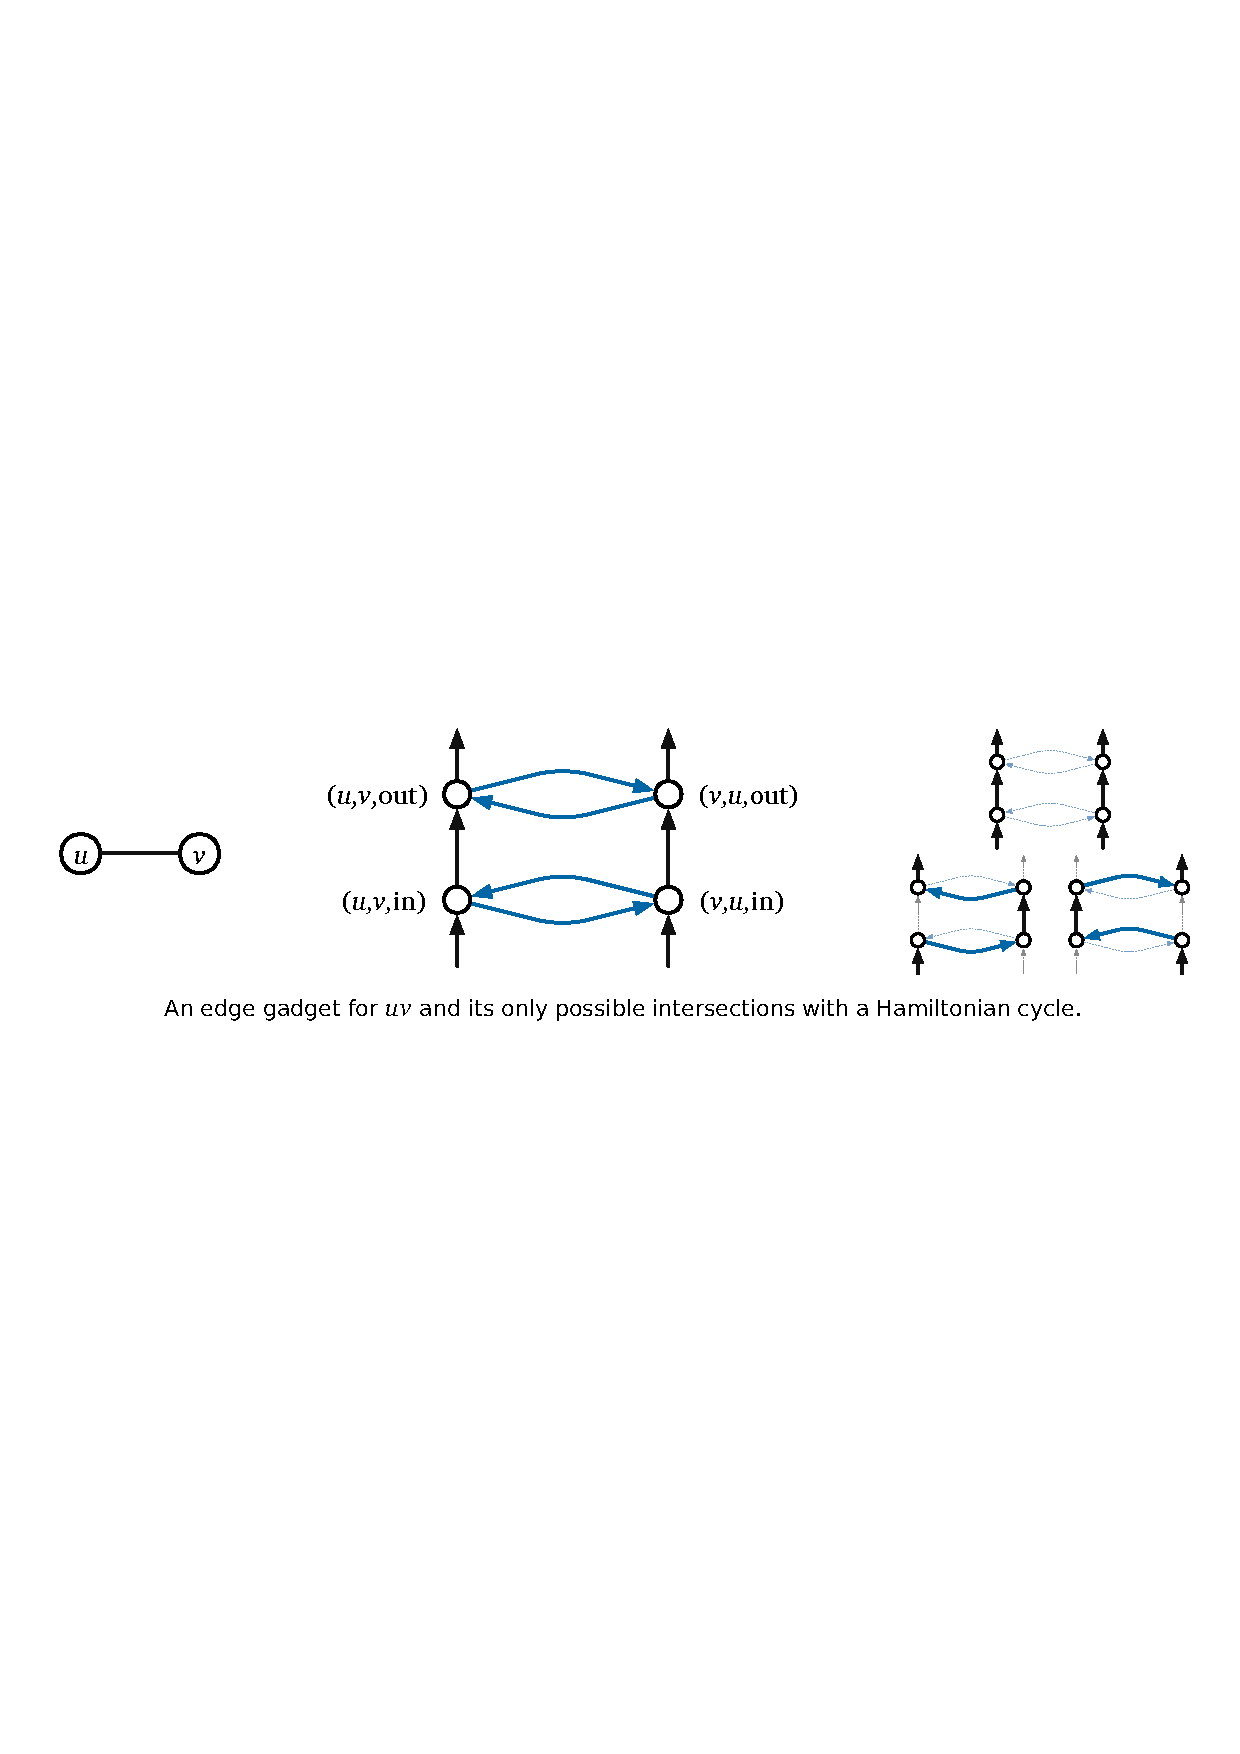
\includegraphics[width=15cm]{figures/hamiltonian.pdf}}
\source{Jeff Erickson, Algorithms etc, NP-Hard Problems}

\section{Règle de chantier}

On vous donne une règle de chantier qui consiste en $n$ bandes de bois, de largeur $2cm$, et reliées entre eux de manière séquentielle par des rivets à $1cm$ de chaque extrémité. La $i$-ième bande a une longueur de $a_i>2$ cm pour $a_i$ entier.

Le but est de la replier pour qu'elle entre sans dépasser dans une boite de $2$cm de haut et de $B$ cm de long, et assez large.
On veut montrer que \textsc{Règle de chantier} est NP-complet, par réduction de \textsc{2-Partition}.

\centerline{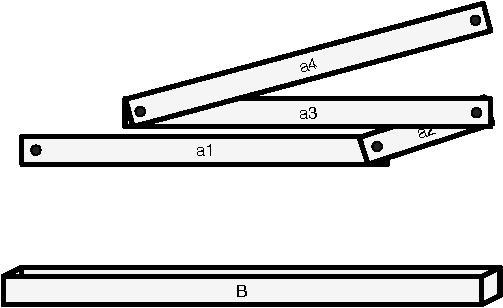
\includegraphics[width=9cm]{figures/regle.pdf}}


\newpage
\section{Jeu de Cubic}
\noindent \textbf{Définition.} Cubic \textit{est un jeu à un joueur qui se joue sur une grille de carrés. Il existe trois types de carrés:}
\begin{itemize}
\item \textit{les murs (représentés en noir): ceux-ci ne peuvent pas être déplacer,}
\item \textit{les cases vides (représentées en blanc),}
\item \textit{les blocs de couleur (représentés en gris, la couleur est représentée par un nombre).}
\end{itemize}
\textit{A chaque tour, le joueur peut déplacer un bloc de couleur d'une case vers la gauche ou d'une case vers la droite, si les cases correspondantes ne sont pas déjà occupées par un mur ou un autre bloc de couleur. Si un bloc de couleur se trouve au dessus d'une case vide, il "tombe" jusqu'à rencontrer un mur ou un bloc de couleur. Si deux blocs de la même couleur partage un côté, ils disparaissent. Éventuellement, les blocs de couleur se trouvant au dessus-eux tombent. Le joueur gagne s'il arrive à faire disparaitre tous les blocs de couleur.}

\begin{figure}[p]
\begin{center}
  \begin{tabular}{c c}
    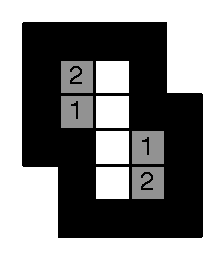
\includegraphics[scale=0.65]{./figures/exemple1} &
    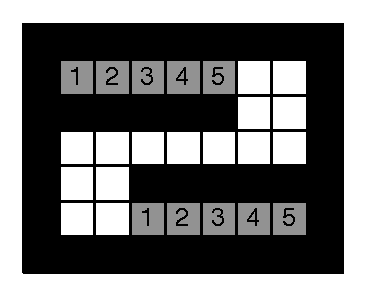
\includegraphics[scale=0.65]{./figures/exemple2}\\
 jeu $1$ &
 jeu $2$
 \end{tabular}
\end{center}
 \caption{Deux configurations initiales du jeu \textit{Cubic}.}
 \label{exemples}
\end{figure}

\begin{enumerate}
	\item Résolvez les problèmes de \textit{Cubic} de la figure \ref{exemples}.
\end{enumerate}

Étant donné une instance de \textit{Cubic}, nous souhaitons déterminer si celle-ci admet une solution. Nous allons montrer que ce problème est NP-complet. Pour cela, nous allons effectuer une réduction à partir de SAT.


\begin{figure}[p]
\begin{center}
  \begin{tabular}{c c}
    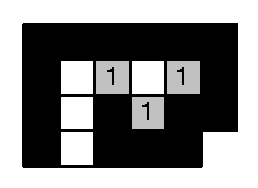
\includegraphics[scale=0.65]{./figures/variable} &
    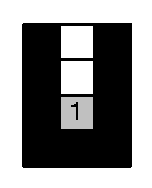
\includegraphics[scale=0.65]{./figures/fil}\\
 encodage d'une variable &
 encodage de la sortie
 \end{tabular}
\end{center}
 \caption{Encodage des variables et de la sortie.}
 \label{debutfin}
\end{figure}

\begin{enumerate}
\item[2.] Exprimez le problème SAT sous la forme de circuit (graphe orienté où les sommets représentent des opérateurs logiques et tous les arcs sont orientés du haut vers le bas).
\end{enumerate}

Nous allons transformer une instance de SAT encodée sous forme de circuit en une instance de \textit{Cubic} qui admet une solution si et seulement si le circuit admet une affectation des variables qui donne une sortie VRAI. On encode les variables et les sorties comme indiqué dans la figure~\ref{debutfin}.


\begin{enumerate}
\item[3.] Expliquez comme fonctionne cette encodage. De quels autres gadgets a-t-on besoin?
\end{enumerate}


\begin{figure}[h]
\begin{center}
  \begin{tabular}{c c c}
    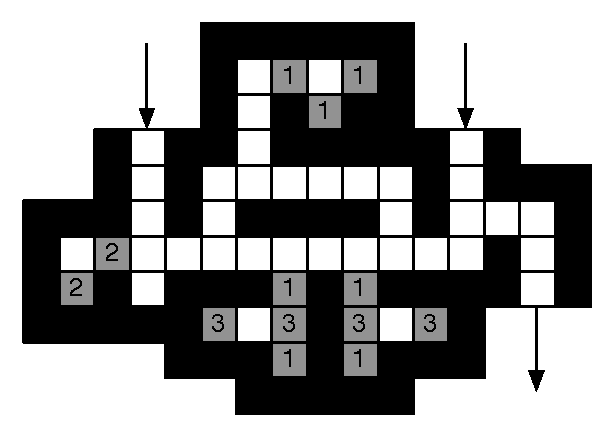
\includegraphics[scale=0.58]{./figures/porteAND} &
    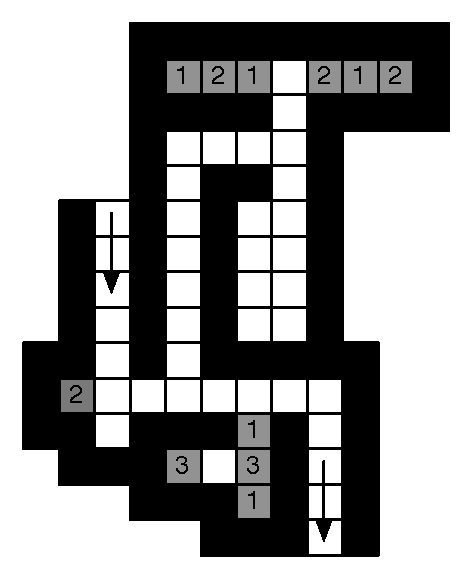
\includegraphics[scale=0.58]{./figures/porteSWITCH} &
    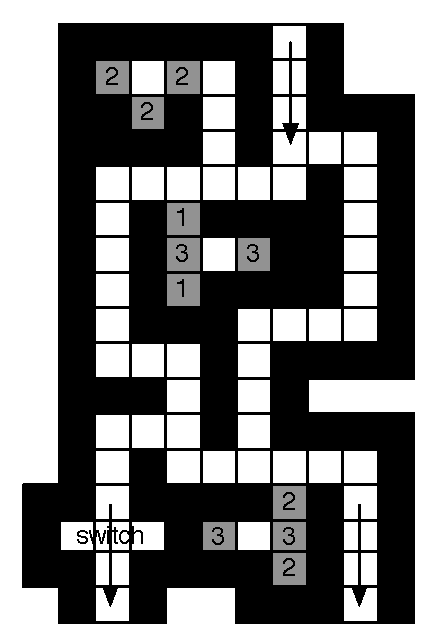
\includegraphics[scale=0.58]{./figures/porteMYSTERE}\\
 porte AND &
 porte SWITCH &
 porte mystère
 \end{tabular}
\end{center}
 \caption{Différents gadgets.}
 \label{gadgets}
\end{figure}

\begin{enumerate}
	\setcounter{enumi}{3}
	\item Expliquez le fonctionnement de la porte AND de la figure \ref{gadgets}.
	\item Expliquez comment faire une porte NOT et une porte OR.
	\item A quoi sert la construction SWITCH de la figure \ref{gadgets}.
	\item En utilisant la structure SWITCH, créez une structure faisant un croisement de fils.
	\item Que fait la construction mystère de la figure \ref{gadgets}.
	\item Montrez que \textit{Cubic} est NP-complet.
\end{enumerate}

\source{https://www2.stetson.edu/\~{}efriedma/papers/spiral.ppt}

\end{document}